\section{Wyznaczenie wektorów $s$ i $s_z$ }
\label{projekt:zad3}

\subsection{Wyznaczenie wektora $s$}
\label{projekt:zad3:s}

Uzyskaną odpowiedź procesu na zmianę sygnału sterującego z punktu pracy Upp=32 na
Umax=55 przekształcono w następujący sposób: 
\begin{itemize}
    \item Ograniczono (przycięto) czas zmiany sterowania u oraz wyjścia y od chwili skoku do ustabilizowania, 
    \begin{itemize}
        \item subsec
    \end{itemize}
    \item Wykres sterowania u przesunięty został o wartość początkową Upp=? w dół, 
    \item Wykres wyjścia y przesunięty został o wartość początkową Ypp=? w dół, 
    \item Wykres sterowania u i wyjścia y podzielono przez delta u=23. 
\end{itemize}

Uzyskana odpowiedź skokowa daje nam zestaw liczb s1,s2. . . ,która wykorzystana będzie w algorytmie DMC.

\begin{figure}[H] 
    \centering
    % This file was created by matlab2tikz.
%
\definecolor{mycolor1}{rgb}{0.00000,0.44700,0.74100}%
%
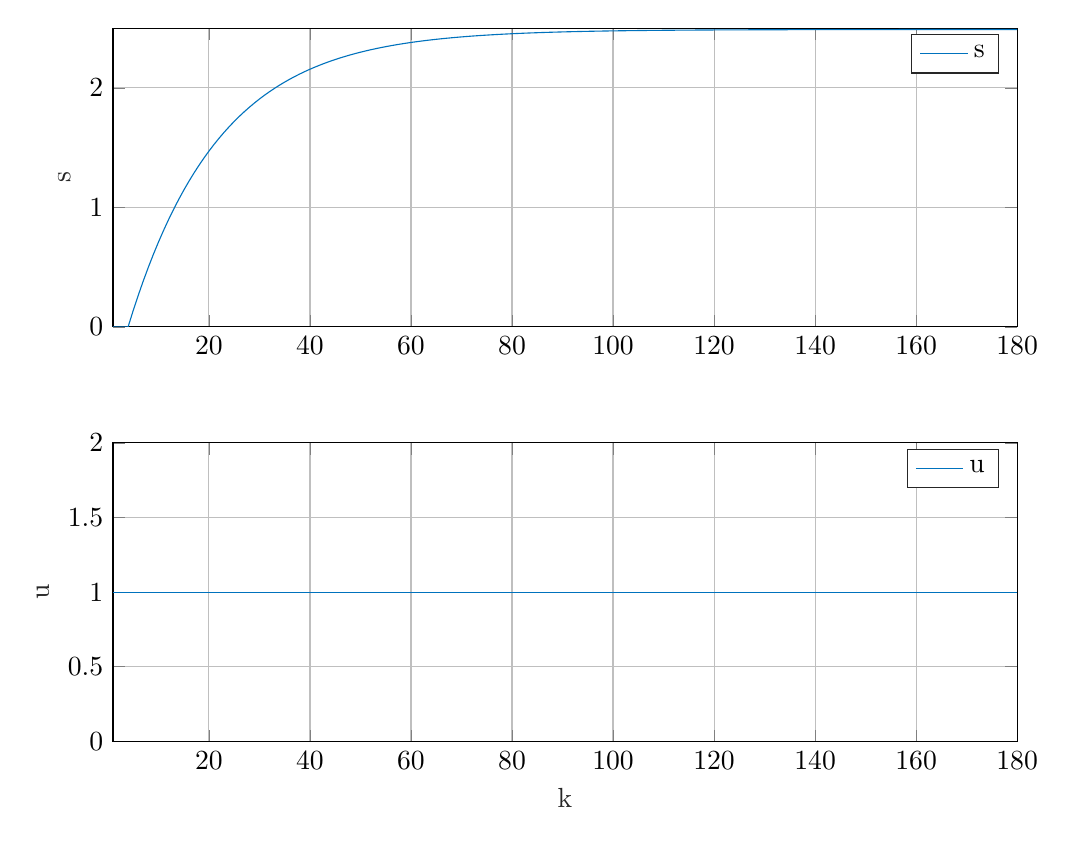
\begin{tikzpicture}

\begin{axis}[%
width=4.521in,
height=1.493in,
at={(0.758in,2.554in)},
scale only axis,
xmin=1,
xmax=180,
ymin=0,
ymax=2.5,
ylabel style={font=\color{white!15!black}},
ylabel={s},
axis background/.style={fill=white},
xmajorgrids,
ymajorgrids,
legend style={legend cell align=left, align=left, draw=white!15!black}
]
\addplot [color=mycolor1]
  table[row sep=crcr]{%
1	0\\
2	0\\
3	0\\
4	0\\
5	0.1351\\
6	0.26289\\
7	0.38377\\
8	0.49811\\
9	0.60625\\
10	0.70854\\
11	0.80528\\
12	0.89678\\
13	0.98332\\
14	1.0652\\
15	1.1426\\
16	1.2158\\
17	1.285\\
18	1.3505\\
19	1.4124\\
20	1.471\\
21	1.5264\\
22	1.5787\\
23	1.6283\\
24	1.6751\\
25	1.7194\\
26	1.7613\\
27	1.8009\\
28	1.8383\\
29	1.8737\\
30	1.9072\\
31	1.9389\\
32	1.9689\\
33	1.9972\\
34	2.024\\
35	2.0493\\
36	2.0732\\
37	2.0959\\
38	2.1173\\
39	2.1375\\
40	2.1567\\
41	2.1748\\
42	2.1919\\
43	2.2081\\
44	2.2234\\
45	2.2379\\
46	2.2516\\
47	2.2645\\
48	2.2768\\
49	2.2883\\
50	2.2993\\
51	2.3096\\
52	2.3194\\
53	2.3286\\
54	2.3374\\
55	2.3457\\
56	2.3535\\
57	2.3609\\
58	2.3679\\
59	2.3745\\
60	2.3807\\
61	2.3866\\
62	2.3922\\
63	2.3975\\
64	2.4025\\
65	2.4072\\
66	2.4117\\
67	2.4159\\
68	2.4199\\
69	2.4237\\
70	2.4273\\
71	2.4307\\
72	2.4339\\
73	2.4369\\
74	2.4397\\
75	2.4424\\
76	2.445\\
77	2.4474\\
78	2.4497\\
79	2.4518\\
80	2.4539\\
81	2.4558\\
82	2.4576\\
83	2.4594\\
84	2.461\\
85	2.4625\\
86	2.464\\
87	2.4654\\
88	2.4667\\
89	2.4679\\
90	2.4691\\
91	2.4702\\
92	2.4712\\
93	2.4722\\
94	2.4731\\
95	2.474\\
96	2.4749\\
97	2.4756\\
98	2.4764\\
99	2.4771\\
100	2.4778\\
101	2.4784\\
102	2.479\\
103	2.4795\\
104	2.4801\\
105	2.4806\\
106	2.4811\\
107	2.4815\\
108	2.4819\\
109	2.4823\\
110	2.4827\\
111	2.4831\\
112	2.4834\\
113	2.4837\\
114	2.484\\
115	2.4843\\
116	2.4846\\
117	2.4849\\
118	2.4851\\
119	2.4853\\
120	2.4856\\
121	2.4858\\
122	2.486\\
123	2.4861\\
124	2.4863\\
125	2.4865\\
126	2.4866\\
127	2.4868\\
128	2.4869\\
129	2.487\\
130	2.4872\\
131	2.4873\\
132	2.4874\\
133	2.4875\\
134	2.4876\\
135	2.4877\\
136	2.4878\\
137	2.4879\\
138	2.4879\\
139	2.488\\
140	2.4881\\
141	2.4882\\
142	2.4882\\
143	2.4883\\
144	2.4883\\
145	2.4884\\
146	2.4884\\
147	2.4885\\
148	2.4885\\
149	2.4886\\
150	2.4886\\
151	2.4887\\
152	2.4887\\
153	2.4887\\
154	2.4888\\
155	2.4888\\
156	2.4888\\
157	2.4889\\
158	2.4889\\
159	2.4889\\
160	2.4889\\
161	2.4889\\
162	2.489\\
163	2.489\\
164	2.489\\
165	2.489\\
166	2.489\\
167	2.4891\\
168	2.4891\\
169	2.4891\\
170	2.4891\\
171	2.4891\\
172	2.4891\\
173	2.4891\\
174	2.4891\\
175	2.4892\\
176	2.4892\\
177	2.4892\\
178	2.4892\\
179	2.4892\\
180	2.4892\\
};
\addlegendentry{s}

\end{axis}

\begin{axis}[%
width=4.521in,
height=1.493in,
at={(0.758in,0.481in)},
scale only axis,
xmin=1,
xmax=180,
xlabel style={font=\color{white!15!black}},
xlabel={k},
ymin=-0,
ymax=2,
ylabel style={font=\color{white!15!black}},
ylabel={u},
axis background/.style={fill=white},
xmajorgrids,
ymajorgrids,
legend style={legend cell align=left, align=left, draw=white!15!black}
]
\addplot[const plot, color=mycolor1] table[row sep=crcr] {%
1	1\\
2	1\\
3	1\\
4	1\\
5	1\\
6	1\\
7	1\\
8	1\\
9	1\\
10	1\\
11	1\\
12	1\\
13	1\\
14	1\\
15	1\\
16	1\\
17	1\\
18	1\\
19	1\\
20	1\\
21	1\\
22	1\\
23	1\\
24	1\\
25	1\\
26	1\\
27	1\\
28	1\\
29	1\\
30	1\\
31	1\\
32	1\\
33	1\\
34	1\\
35	1\\
36	1\\
37	1\\
38	1\\
39	1\\
40	1\\
41	1\\
42	1\\
43	1\\
44	1\\
45	1\\
46	1\\
47	1\\
48	1\\
49	1\\
50	1\\
51	1\\
52	1\\
53	1\\
54	1\\
55	1\\
56	1\\
57	1\\
58	1\\
59	1\\
60	1\\
61	1\\
62	1\\
63	1\\
64	1\\
65	1\\
66	1\\
67	1\\
68	1\\
69	1\\
70	1\\
71	1\\
72	1\\
73	1\\
74	1\\
75	1\\
76	1\\
77	1\\
78	1\\
79	1\\
80	1\\
81	1\\
82	1\\
83	1\\
84	1\\
85	1\\
86	1\\
87	1\\
88	1\\
89	1\\
90	1\\
91	1\\
92	1\\
93	1\\
94	1\\
95	1\\
96	1\\
97	1\\
98	1\\
99	1\\
100	1\\
101	1\\
102	1\\
103	1\\
104	1\\
105	1\\
106	1\\
107	1\\
108	1\\
109	1\\
110	1\\
111	1\\
112	1\\
113	1\\
114	1\\
115	1\\
116	1\\
117	1\\
118	1\\
119	1\\
120	1\\
121	1\\
122	1\\
123	1\\
124	1\\
125	1\\
126	1\\
127	1\\
128	1\\
129	1\\
130	1\\
131	1\\
132	1\\
133	1\\
134	1\\
135	1\\
136	1\\
137	1\\
138	1\\
139	1\\
140	1\\
141	1\\
142	1\\
143	1\\
144	1\\
145	1\\
146	1\\
147	1\\
148	1\\
149	1\\
150	1\\
151	1\\
152	1\\
153	1\\
154	1\\
155	1\\
156	1\\
157	1\\
158	1\\
159	1\\
160	1\\
161	1\\
162	1\\
163	1\\
164	1\\
165	1\\
166	1\\
167	1\\
168	1\\
169	1\\
170	1\\
171	1\\
172	1\\
173	1\\
174	1\\
175	1\\
176	1\\
177	1\\
178	1\\
179	1\\
180	1\\
};
\addlegendentry{u}

\end{axis}
\end{tikzpicture}%
    \caption{Wektor $s$}
    \label{projekt:zad3:s:figure}
\end{figure}

\subsection{Wyznaczenie wektora $s_z$}
\label{projekt:zad3:sz}

Uzyskaną odpowiedź procesu na zmianę sygnału zakłócenia z punktu pracy Zpp=0 na
Zmax =30 przekształcono w następujący sposób: 
\begin{itemize}
\item Ograniczono (przycięto) czas zmiany sterowania u oraz wyjścia y od chwili skoku do ustabilizowania, 
\item Wykres sterowania u przesunięty został o wartość początkową Upp=? w dół, 
\item Wykres wyjścia y przesunięty został o wartość początkową Ypp=? w dół, 
\item Wykres sterowania u i wyjścia y podzielono przez delta z= 30.
\end{itemize}


Uzyskana odpowiedź skokowa toru zakłócenie wyjście daje nam zestaw liczb s1z,s2z. . .
,która wykorzystana będzie w algorytmie DMC.

\begin{figure}[H] 
    \centering
    % This file was created by matlab2tikz.
%
\definecolor{mycolor1}{rgb}{0.00000,0.44700,0.74100}%
%
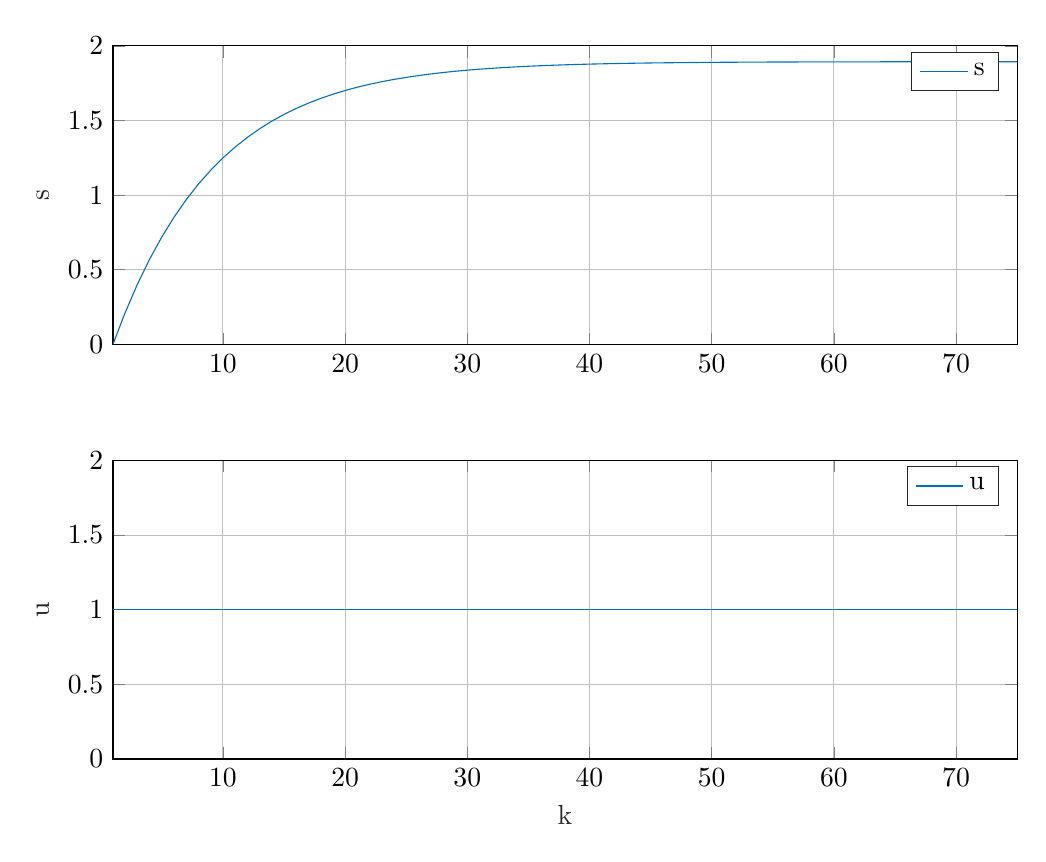
\begin{tikzpicture}

\begin{axis}[%
width=4.521in,
height=1.493in,
at={(0.758in,2.554in)},
scale only axis,
xmin=1,
xmax=75,
ymin=0,
ymax=2,
ylabel style={font=\color{white!15!black}},
ylabel={s},
axis background/.style={fill=white},
xmajorgrids,
ymajorgrids,
legend style={legend cell align=left, align=left, draw=white!15!black}
]
\addplot [color=mycolor1]
  table[row sep=crcr]{%
1	0\\
2	0.21325\\
3	0.40257\\
4	0.57063\\
5	0.71982\\
6	0.85226\\
7	0.96982\\
8	1.0742\\
9	1.1668\\
10	1.249\\
11	1.322\\
12	1.3867\\
13	1.4442\\
14	1.4952\\
15	1.5404\\
16	1.5805\\
17	1.6162\\
18	1.6478\\
19	1.6758\\
20	1.7007\\
21	1.7227\\
22	1.7423\\
23	1.7596\\
24	1.775\\
25	1.7886\\
26	1.8007\\
27	1.8114\\
28	1.8209\\
29	1.8294\\
30	1.8368\\
31	1.8434\\
32	1.8493\\
33	1.8545\\
34	1.859\\
35	1.8631\\
36	1.8667\\
37	1.8699\\
38	1.8727\\
39	1.8752\\
40	1.8774\\
41	1.8793\\
42	1.881\\
43	1.8826\\
44	1.8839\\
45	1.8851\\
46	1.8861\\
47	1.887\\
48	1.8878\\
49	1.8886\\
50	1.8892\\
51	1.8897\\
52	1.8902\\
53	1.8907\\
54	1.891\\
55	1.8914\\
56	1.8916\\
57	1.8919\\
58	1.8921\\
59	1.8923\\
60	1.8925\\
61	1.8926\\
62	1.8927\\
63	1.8928\\
64	1.8929\\
65	1.893\\
66	1.8931\\
67	1.8931\\
68	1.8932\\
69	1.8932\\
70	1.8933\\
71	1.8933\\
72	1.8933\\
73	1.8934\\
74	1.8934\\
75	1.8934\\
};
\addlegendentry{s}

\end{axis}

\begin{axis}[%
width=4.521in,
height=1.493in,
at={(0.758in,0.481in)},
scale only axis,
xmin=1,
xmax=75,
xlabel style={font=\color{white!15!black}},
xlabel={k},
ymin=-0,
ymax=2,
ylabel style={font=\color{white!15!black}},
ylabel={u},
axis background/.style={fill=white},
xmajorgrids,
ymajorgrids,
legend style={legend cell align=left, align=left, draw=white!15!black}
]
\addplot[const plot, color=mycolor1] table[row sep=crcr] {%
1	1\\
2	1\\
3	1\\
4	1\\
5	1\\
6	1\\
7	1\\
8	1\\
9	1\\
10	1\\
11	1\\
12	1\\
13	1\\
14	1\\
15	1\\
16	1\\
17	1\\
18	1\\
19	1\\
20	1\\
21	1\\
22	1\\
23	1\\
24	1\\
25	1\\
26	1\\
27	1\\
28	1\\
29	1\\
30	1\\
31	1\\
32	1\\
33	1\\
34	1\\
35	1\\
36	1\\
37	1\\
38	1\\
39	1\\
40	1\\
41	1\\
42	1\\
43	1\\
44	1\\
45	1\\
46	1\\
47	1\\
48	1\\
49	1\\
50	1\\
51	1\\
52	1\\
53	1\\
54	1\\
55	1\\
56	1\\
57	1\\
58	1\\
59	1\\
60	1\\
61	1\\
62	1\\
63	1\\
64	1\\
65	1\\
66	1\\
67	1\\
68	1\\
69	1\\
70	1\\
71	1\\
72	1\\
73	1\\
74	1\\
75	1\\
};
\addlegendentry{u}

\end{axis}
\end{tikzpicture}%
    \caption{Wektor $s_{z}$}
    \label{projekt:zad3:sz:figure}
\end{figure}
